% Chapter Template

\chapter{LegoOS} % Main chapter title

\label{ChapterX} % Change X to a consecutive number; for referencing this chapter elsewhere, use \ref{ChapterX}

%----------------------------------------------------------------------------------------
%	SECTION 1
%----------------------------------------------------------------------------------------

\section{研究背景}

现阶段,数据中心的部署、执行、故障单元等都是一整台的物理服务器(monolithic server),这台服务器包含了运行一个程序所需要的全部硬件资源(CPU、内存、磁盘等)。但是,这种架构使得硬件资源很难得到充分的利用。例如,不同的应用程序对于资源占用的侧重不同:一些计算密集型的程序对CPU要求很高,但是不需要占用很多内存;而一些数据存储服务程序则要求磁盘和网络具有较大的吞吐量,而CPU性能则其次。单台完整的服务器无法完美适配不同的程序对于资源的使用。另外,即使服务器只有一个硬件组件故障,也会使整体不可用。

硬件资源分解(hardware resource disaggregation)是一种新的技术,把不同的硬件设备组织为独立的组件,组件之间依靠网络进行通信而不是集中在一台服务器中。这样可以最大化硬件资源的利用率,弹性装配,还能够隔离硬件之间的故障。

%----------------------------------------------------------------------------------------
%	SECTION 2
%----------------------------------------------------------------------------------------

\section{相关研究和挑战}
\begin{itemize}
\item 硬件发展:首先,网络的速度越来越快,在逐步接近内存总线的数量级,这使得基于网络的硬件通信在性能上成为可能。其次,硬件设备的功能越发丰富,因而可以直接在硬件上实现控制器、处理网络请求等,无需软件的辅助。
\item 内存分离:基于RDMA技术(远程直接内存访问),目前已有大量远程内存利用的研究。例如,在一个集群中,内存负载大的服务器可以把一些页面交换到内存负载轻的服务器上而不是本地磁盘,从而获得更高的效率。\parencite{gu2017efficient}
\item 存储分离:有关分布式存储的研究十分丰富,而且已经大规模的部署在了云服务商的机器上。
\item 多内核操作系统:一些操作系统在每个CPU核心上运行一个小的kernel,并使用消息机制通信。这样,运行在任何物理核心上的kernel代码都可以快速替换。\parencite{zellweger2014decoupling}
\end{itemize}

以上研究已经分别实现了内存、存储、核心等的分离,但OS主体仍然运行在monolithic server上,OS仍然需要管理不同的硬件资源(CPU,内存,和存储等)。LegoOS是全新设计的体系结构。与传统的基于monolithic server的方案相比,它能够真正完全分离硬件资源,每个组件(component)只管理属于自己的硬件资源(CPU,内存,或存储中的一个)。例如,管理CPU的组件将没有本地的内存和存储,而是通过网络与内存组件和存储组件通信。这样做可以实现内存和CPU等资源的完全利用,而且方便随时添加和移除硬件组件,甚至是完全异构的硬件;进一步的,硬件故障的影响范围被局限在了每个独立的硬件组件而不是整台服务器。这些优点是monolithic server的方案所无法做到的。

当然,这带来了许多挑战:在组件之间的网络通信速度达不到总线的速度时,如何保证提供良好的性能;如何协调与管理所有独立的组件;如何确保一个组件的failure不影响到其他组件;如何兼容现有应用;等。

%----------------------------------------------------------------------------------------
%	SECTION 3
%----------------------------------------------------------------------------------------

\section{架构和设计}

LegoOS在设计上针对三种硬件组件:处理器、内存、存储,分别称为pComponent、mComponent、sComponent。在接口方面,LegoOS暴露给用户的是一组vNode。每个vNode有自己独立的IP,可以运行多个pComponent、mComponent、sComponent。LegoOS确保每个vNode的资源相互之间完全隔离。LegoOS实现了大多数的Linux system call接口,使得大多数程序可以未修改的在LegoOS的一组vNode上运行。

%-----------------------------------
%	SUBSECTION 1
%-----------------------------------
\subsection{处理器管理}

\begin{figure}[h]
\centering
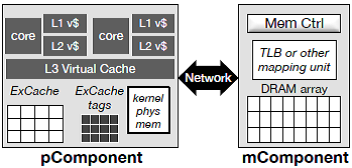
\includegraphics[scale=1.00]{Figures/legoos/1.png}
\decoRule
\caption{LegoOS pComponent and mComponent Archiecture}
\label{fig:legoos_archiecture}
\end{figure}

pComponent专门管理处理器内核。它使用了针对数据中心程序的一个简单的调度模型。每个pComponent为内核线程保留少量的核心,然后分配其他的核心给用户线程。并且,尽量减少线程调度和内核抢占以提高性能(例如,不使用中断而是用轮询处理网络请求,由于网络延迟在LegoOS中很低)。

pComponent完全不需要地址映射,mmu和TLB等完全由mComponent维护。在本地,pComponent只持有少量的内存缓存,称为ExCache,位于处理器的Last-Level Cache(LLC)之下。每个ExCache line有一个虚拟地址的tag和两个标记位(P,R/W),由软件设置、硬件检查。当ExCache miss时,LegoOS通过网络从对应的mComponent中取回数据填入ExCache line中。ExCache miss的处理甚至可以完全由硬件实现以获得最高的效率。

%-----------------------------------
%	SUBSECTION 2
%-----------------------------------

\subsection{内存管理}

\begin{figure}[h]
\centering
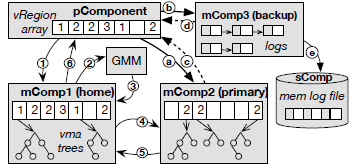
\includegraphics[scale=1.00]{Figures/legoos/2.png}
\decoRule
\caption{LegoOS Distributed Memory Management}
\label{fig:legoos_memory_management}
\end{figure}

mComponent管理虚拟内存和物理内存,包括它们的分配、回收和映射。这里采用了两级的内存管理。在high level,把虚拟地址空间粗粒度的划分为了固定大小的vRegions,每个已被分配的vRegion都被一个mComponent管理。在low level,mComponent记录了每个vRegion上分配给用户的vma树。

当用户程序申请虚拟内存空间时,pComponent把相关的请求转发给对应的mComponent。mComponent会查询自己管理vRegions,寻找一个合适的vRegion来为用户分配内存。如果可用虚拟内存空间不足,还会向全局的内存资源管理器GMM申请一个新的vRegion并把请求转发到另一个mComponent。pComponent也会缓存用户程序的vRegion array。

考虑到内存故障的可能性与影响更大,LegoOS对mComponent提供了可靠性保证。当pComponent刷新ExCache时,消息被同时发往primary mComponnet和对应的backup mComponent。其中primary mComponent维护内存数据和元数据,backup mComponent在后台把内存操作写入由sComponent管理的append-only log中,这样可以在失败时通过log恢复内存内容。

%-----------------------------------
%	SUBSECTION 3
%-----------------------------------

\subsection{存储管理}

LegoOS在sComponent上实现存储功能。类似于NFS,存储服务器采用无状态的设计,并通过vNode抽象后暴露给用户。用户可以通过标准POSIX api操作vNode上的挂载点,从而访问存储系统。

由于sComponent的内部内存有限,LegoOS在mComponent上放置存储缓冲区。当用户通过系统调用访问文件时,抽象层把请求的文件完整路径、偏移量和大小转发给mComponent,mComponent查找缓冲区,并在需要时从sComponent获取缺失的数据以及将文件数据sync到sComponent中。

%----------------------------------------------------------------------------------------
%	SECTION 4
%----------------------------------------------------------------------------------------

\section{本章小结}

LegoOS是第一个为了硬件资源分离而设计的操作系统,它将一个操作系统管理不同硬件的功能分解开。相比于monolithic server,LegoOS可以达到更有效的资源利用率、更高的故障隔离性以及更好的硬件资源弹性。测试和评估表明,经过优化的LegoOS有着很低的网络延迟和较好的内存吞吐量,以及更长的平均无故障时间(MTTF)。而且,随着硬件功能的进一步丰富,一些componnent监视器的逻辑可以由硬件完成,从而进一步提高性能。
